\section{Q2-4}
\emph{Draw a use case diagram for a ticket distributor for a train system. The system includes two actors: a traveler who purchases different types of tickets, and a central computer system that maintains a reference database for the tariff. Use cases should include
BuyOneWayTicket, BuyWeeklyCard, BuyMonthlyCard, and UpdateTariff. Also include the following exceptional cases: TimeOut (i.e., traveler took too long to insert the right amount), TransactionAborted (i.e., traveler selected the cancel button without completing the transaction), DistributorOutOfChange, and DistributorOutOfPaper.}
\\
\emph{Remember that a use case diagram consists of both the sticky man diagram as well as the use cases written in text using the template on p. 45 in OOSE. }
\\
\emph{Use Case Diagram - Use Case}
\\
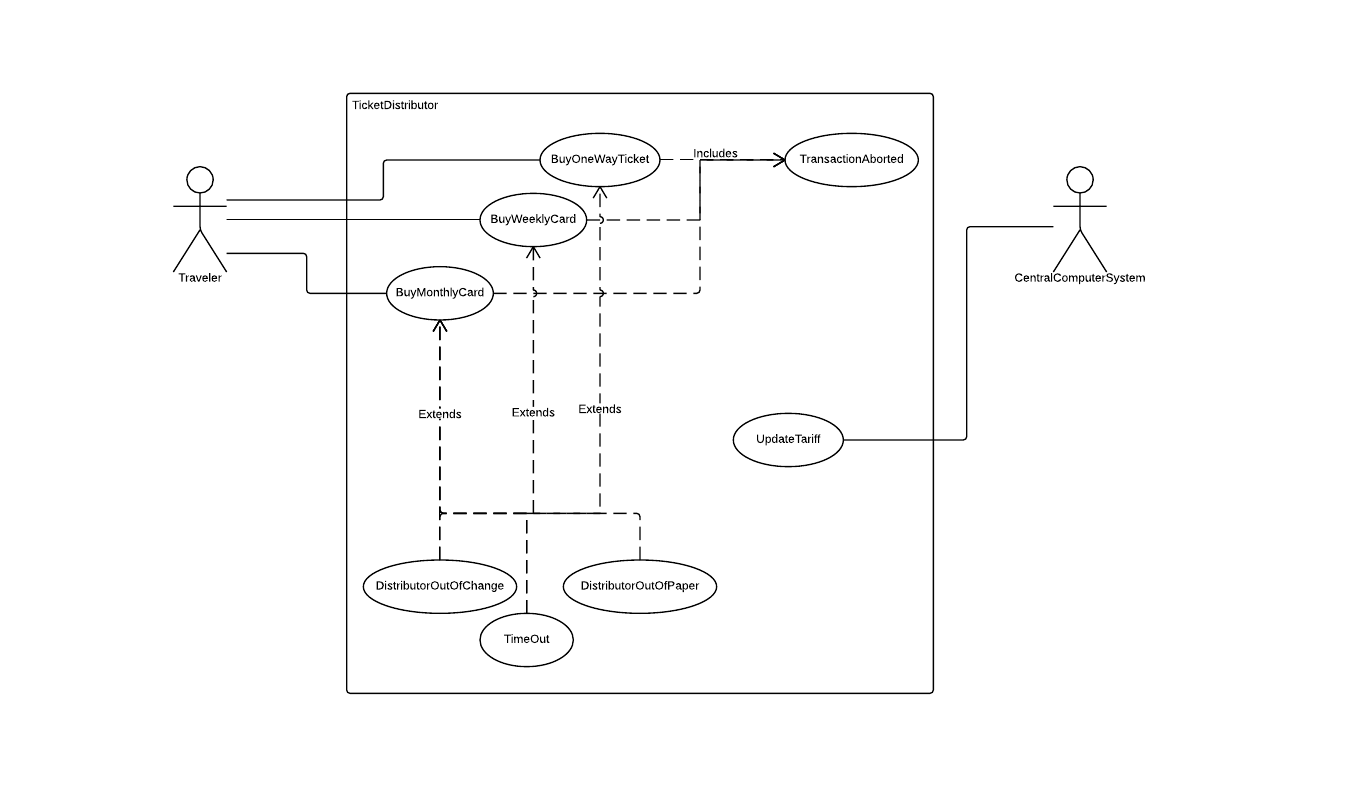
\includegraphics[scale=0.3]{Assignment-36-Use-Case-Diagram-Use-Case}

\HRule \\[0.4cm]

\textbf{Use case name:} BuyTicket

\HRule \\[0.4cm]

\textbf{Participating actors:}
\begin{itemize}
	\item Initiated by Traveler
	\item Communicates with CentralComputerSystem
\end{itemize}

\HRule \\[0.4cm]

\textbf{Flow of events:}
\begin{enumerate}
	\item Traveler initiates BuyOneWayTicket, BuyWeeklyCard or BuyMonthlyCard.
	\item Traveler pays for the ticket.
	\begin{enumerate}
		\item (Exceptional case) Timeout: Traveler took too long to insert the right amount of money. TicketDistributor has to abort.
		\item (Exceptional case) TransactionAborted: Traveler selected the cancel button without completing the transaction.
		\item (Exceptional case) DistributorOutOfChange: TicketDistributor is out of change, and can therefore not give back change to the Traveler, and has to abort.
		\item (Exceptional case) DistributorOutOfPaper: TicketDistributor is out of paper, and can therefore not print out the ticket for the Traveler, and has to abort.
	\end{enumerate}
	\item UpdateTariff is initiated, and the database is being updated.
\end{enumerate}

\HRule \\[0.4cm]

\textbf{Entry condition:} Traveler interacts with the TicketDistributor.

\HRule \\[0.4cm]

\textbf{Exit condition:}
\begin{itemize}
	\item Traveler has received the ticket and change (if any).
	\item Traveler has initiated TransactionAborted.
	\item TicketDistributor has initiated DistributorOutOfChange OR DistributorOutOfPaper.
\end{itemize}

\HRule \\[0.4cm]

\textbf{Quality Requirements:}

\HRule \\[0.4cm]
